% !TEX root = ../thesis.tex

\chapter{Evaluation}
\label{evaluation}
\subsection{Models preview}
On the figure~\ref{plot} is graphical presentation of data nad our linear and polynomial models. It seen that the first linear model (blue line), is not
directly corresponding the data, but it copy the trend of the income, this we should see on figure~\ref{prediction} with predicted data to 2020.
\begin{figure}[h!]
    \begin{center}
        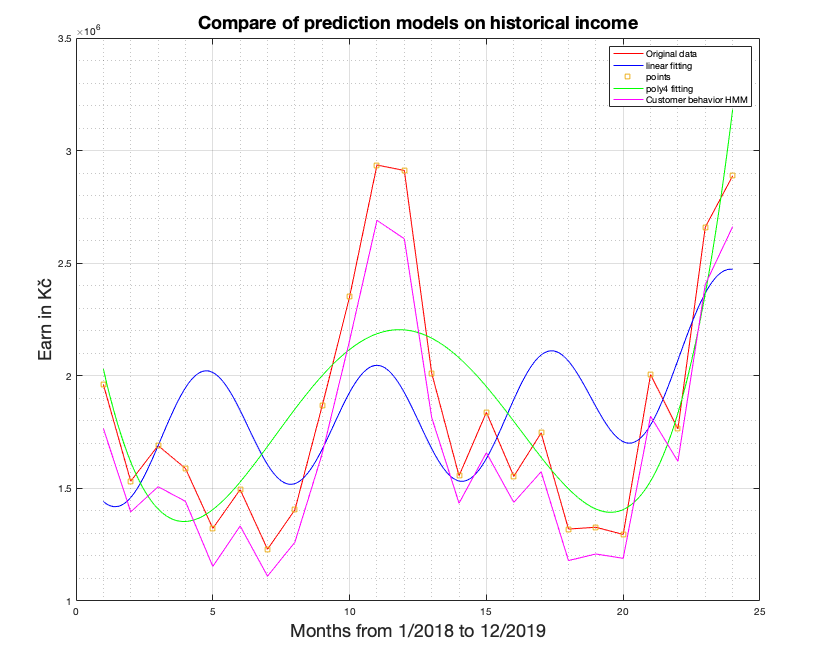
\includegraphics[width=140mm]{plot.png}
    \end{center}
    \caption{Fitting the model on real income from 2018 and 2018}
    \label{plot}
\end{figure}\\
\begin{figure}[h!]
    \begin{center}
        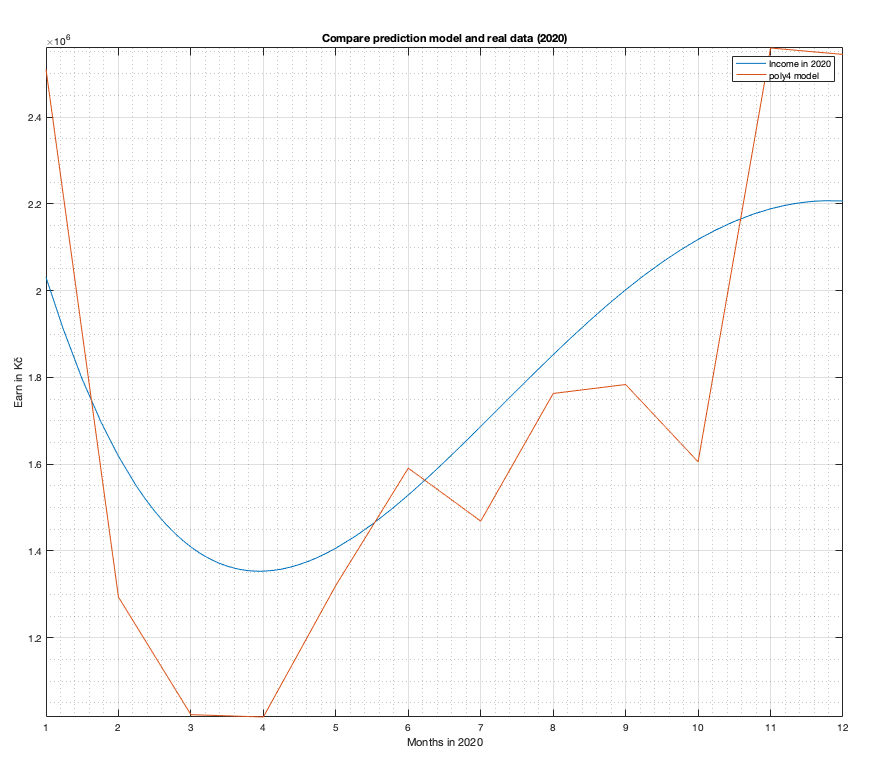
\includegraphics[width=80mm]{polypred.png}
    \end{center}
    \caption{Plot polynomial model to compare with real income in 2020}
    \label{polypred}
\end{figure}\\
\newpage
\subsection{Compare income results}
\begin{table}[h!]
    \begin{center}
        \begin{tabular}{ | l | c | c | c | c | c | c | c |}
            \hline
            {\textbf{Month}} & \textbf{Real income} & \textbf{1st model} & \textbf{(\%)}  & \textbf{2nd model} & \textbf{(\%)} & \textbf{3rd model} & \textbf{(\%)}\\
            \hline
            1/2021 & 2 510 086 & 2 372 333 & 6 & 2 031 000 & 24 & 2 679 419 & 7\\
            2/2021 & 1 293 778 & 2 256 560 & 74 & 1 696 000 & 31 & 1 367 816 & 6\\
            3/2021 & 1 022 762 & 2 340 092 & 129 & 1 409 000 & 38 & 1 092 252 & 7\\
            4/2021 & 1 017 408 & 2 671 671 & 163 & 1 358 000 & 38 & 1 151 301 & 13\\
            5/2021 & 1 320 608 & 3 086 545 & 134 & 1 403 000 & 6 & 1 369 985 & 4\\
            6/2021 & 1 590 878 & 3 359 684 & 111 & 1 511 000 & 5 & 1 632 372 & 3\\
            7/2021 & 1 468 808 & 3 413 621 & 132 & 1 656 000 & 13 & 1 575 324 & 7\\
            8/2021 & 1 762 959 & 3 390 580 & 92 & 1 847 000 & 5 & 1 959 480 & 11\\
            9/2021 & 1 782 582 & 3 522 629 & 98 & 1 987 000 & 11 & 1 950 306 & 9\\
            10/2021 & 1 605 396 & 3 919 220 & 144 & 2 100 000 & 31 & 1 765 984 & 10\\
            11/2021 & 2 559 070 & 4 467 471 & 75 & 2 187 000 & 17 & 2 611 529 & 2\\
            12/2021 & 2 544 271 & 4 936 855 & 94 & 2 197 000 & 16 & 2 610 694 & 3\\
            \hline
        \end{tabular}
    \end{center}
    \caption{Compare results}
    \label{Compare results}
\end{table}\\
On the graphical view we saw that all our models copy the trends of the store income, but some models are easier to calculate, this differences you cen see described in summary~\ref{summary}
\begin{figure}[h!]
    \begin{center}
        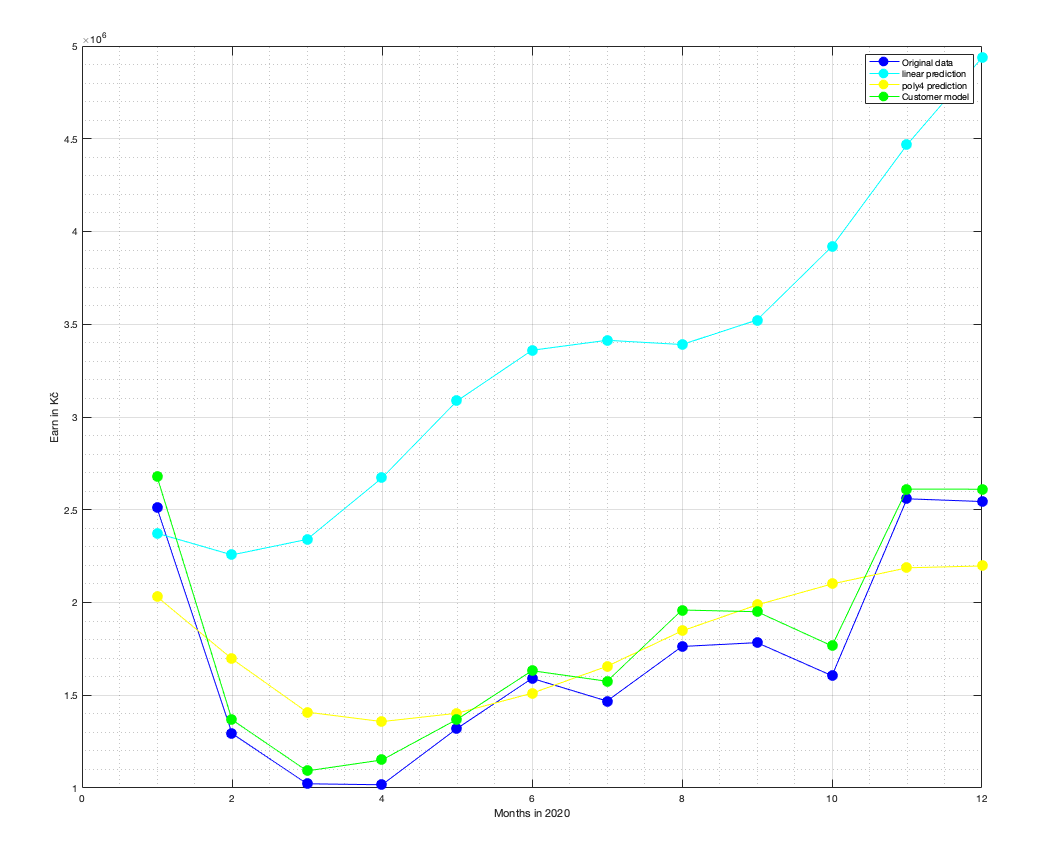
\includegraphics[width=100mm]{prediction.png}
    \end{center}
    \caption{Prediction for year 2020}
    \label{prediction}
\end{figure}\\
\newpage
\subsection{Compare results aberrations} \label{abbr}
\begin{table}[h!]
    \begin{center}
        \begin{tabular}{ | l | c | c | c |}
            \hline
            & \textbf{1st model} & \textbf{2nd model} & \textbf{3rd model}\\
            \hline
            1Q (\%) & 69,66 & 30,81 & 6,42\\
            2Q (\%) & 135,83 & 15,00 & 6,50\\
            3Q (\%) & 107,41 & 9,64 & 9,25\\
            4Q (\%) & 104,25 & 21,21 & 4,89\\
            \hline
        \end{tabular}
    \end{center}
    \caption{Quarterly results}
    \label{qResults}
\end{table}
\newpage
